\documentclass[12pt,a4paper]{article}

\usepackage[utf8]{inputenc}
\usepackage[T5]{fontenc}
\usepackage[vietnamese]{babel}
\usepackage{geometry}
\geometry{left=2.5cm, right=2.0cm, top=2.5cm, bottom=2.5cm}

\usepackage{graphicx}
\usepackage{array}
\usepackage{tabularx}
\usepackage{multirow}
\usepackage{subcaption}
\usepackage{amsmath}
\usepackage{amssymb}
\usepackage{hyperref}
\usepackage{xcolor}
\usepackage{caption}

\hypersetup{
    colorlinks=true,
    linkcolor=blue,
    urlcolor=blue,
    citecolor=blue
}

\setlength{\parindent}{0pt}
\setlength{\parskip}{4pt}

\begin{document}

% ==============================================================================
\section{Giới thiệu bài toán và tập dữ liệu UIT-VSFC}

\subsection{Đặt vấn đề}
Trong môi trường giáo dục đại học, phản hồi của sinh viên sau mỗi học phần là nguồn thông tin định tính quan trọng giúp giảng viên và nhà trường đánh giá chất lượng giảng dạy, nội dung môn học cũng như cơ sở vật chất. Khi số lượng khảo sát lên tới hàng chục nghìn câu mỗi học kỳ, việc đọc và phân loại thủ công trở nên tốn kém thời gian và dễ chịu ảnh hưởng bởi cảm tính chủ quan. Vì vậy, xây dựng một hệ thống Học máy tự động phân loại cảm xúc văn bản (\textit{Sentiment Analysis}) tiếng Việt có giá trị thực tiễn cao.

Bài toán được phát biểu dưới dạng phân loại văn bản đa lớp (\textit{multi-class text classification}): với đầu vào là một câu phản hồi thô $x$, mô hình cần dự đoán nhãn cảm xúc $y \in \{0, 1, 2\}$, tương ứng với ba lớp:
\begin{itemize}
    \item $y = 0$: \textbf{Tiêu cực} (phản ánh hạn chế về giảng dạy, tài liệu, khối lượng bài tập, cơ sở vật chất\dots).
    \item $y = 1$: \textbf{Trung tính} (nhận xét trung lập, góp ý mang tính xây dựng hoặc không bày tỏ thái độ khen/chê rõ ràng, ví dụ \textit{``em không có ý kiến''}).
    \item $y = 2$: \textbf{Tích cực} (khen ngợi sự nhiệt tình, phương pháp truyền đạt dễ hiểu, kiến thức bổ ích\dots).
\end{itemize}

\subsection{Đặc tả tập dữ liệu UIT-VSFC}
Tập dữ liệu được sử dụng là \textbf{UIT-VSFC} (\textit{Vietnamese Students' Feedback Corpus}), tải trực tiếp từ nguồn công khai trên Hugging Face (\texttt{uitnlp/vietnamese\_students\_feedback}) theo định dạng Parquet. Tập dữ liệu có tổng cộng \textbf{16.175 câu} phản hồi tiếng Việt, được chia sẵn thành 3 tập độc lập: tập huấn luyện (\texttt{Train}) gồm 11.426 mẫu, tập kiểm định (\texttt{Validation}) gồm 1.583 mẫu và tập kiểm thử (\texttt{Test}) gồm 3.166 mẫu. Việc giữ nguyên cách chia chuẩn của bộ dữ liệu giúp đảm bảo tính công bằng khi đối chiếu mô hình và loại trừ nguy cơ rò rỉ dữ liệu (\textit{data leakage}).

% ==============================================================================
\section{Phân tích khám phá dữ liệu (EDA)}

\subsection{Thống kê tổng quan và kiểm tra chất lượng dữ liệu}
Trước khi xây dựng mô hình, dữ liệu trên cả 3 tập được kiểm tra giá trị thiếu (\textit{missing values}), chuỗi rỗng, mẫu trùng lặp nội bộ và mẫu trùng lặp chéo giữa các tập. Kết quả tổng hợp trong Bảng~\ref{tab:text_eda_overview} cho thấy dữ liệu rất sạch: không có bất kỳ mẫu nào bị thiếu văn bản, thiếu nhãn hay chứa chuỗi rỗng; tập \texttt{Train} chỉ có duy nhất 1 câu trùng văn bản (0 mẫu trùng đồng thời cả văn bản và nhãn); đặc biệt số câu trùng lặp giữa \texttt{Train--Val} và giữa \texttt{Train--Test} đều bằng \textbf{0}.

\begin{table}[htbp]
\centering
\caption{Thống kê tổng quan và phân phối nhãn trên 3 tập dữ liệu UIT-VSFC}
\label{tab:text_eda_overview}
\scriptsize
\setlength{\tabcolsep}{4pt}
\resizebox{\textwidth}{!}{%
\begin{tabular}{|l|r|r|r|r|r|r|}
\hline
\textbf{Tập dữ liệu} & \textbf{Số mẫu} & \textbf{Thiếu / Rỗng} & \textbf{Trùng text} & \textbf{Tiêu cực (\%)} & \textbf{Trung tính (\%)} & \textbf{Tích cực (\%)} \\
\hline
Train      & 11.426 & 0 / 0 & 1 & 5.325 (46,60\%) & 458 (4,01\%) & 5.643 (49,39\%) \\
\hline
Validation & 1.583  & 0 / 0 & 0 & 705 (44,54\%)   & 73 (4,61\%)  & 805 (50,85\%)   \\
\hline
Test       & 3.166  & 0 / 0 & 0 & 1.409 (44,50\%) & 167 (5,27\%) & 1.590 (50,22\%) \\
\hline
\end{tabular}%
}
\end{table}

\subsection{Phân phối nhãn và vấn đề mất cân bằng lớp}
Từ Bảng~\ref{tab:text_eda_overview} và Hình~\ref{fig:text_label_dist}, có thể nhận thấy một đặc điểm cốt lõi của UIT-VSFC là \textbf{mất cân bằng lớp nghiêm trọng}: hai lớp \textit{Tích cực} ($\sim 49{,}4\% - 50{,}9\%$) và \textit{Tiêu cực} ($\sim 44{,}5\% - 46{,}6\%$) chiếm gần 95\% dữ liệu, trong khi lớp \textbf{Trung tính} chỉ chiếm vỏn vẹn \textbf{4,01\%} ở tập \texttt{Train}, \textbf{4,61\%} ở tập \texttt{Validation} và \textbf{5,27\%} ở tập \texttt{Test}.

Hệ quả trực tiếp là nếu chỉ đánh giá bằng \textbf{Accuracy}, một mô hình dự đoán sai hoàn toàn lớp \textit{Trung tính} vẫn có thể đạt $\sim 90\%$ độ chính xác. Do đó, nghiên cứu này sử dụng \textbf{Macro F1-score} làm thước đo so sánh chính (đặt trọng số ngang nhau cho cả 3 lớp), kết hợp theo dõi \textbf{F1 (Trung tính)} và áp dụng các kỹ thuật cân bằng trọng số lớp (\texttt{class\_weight='balanced'} hoặc trọng số trong hàm mất mát).

\begin{figure}[htbp]
    \centering
    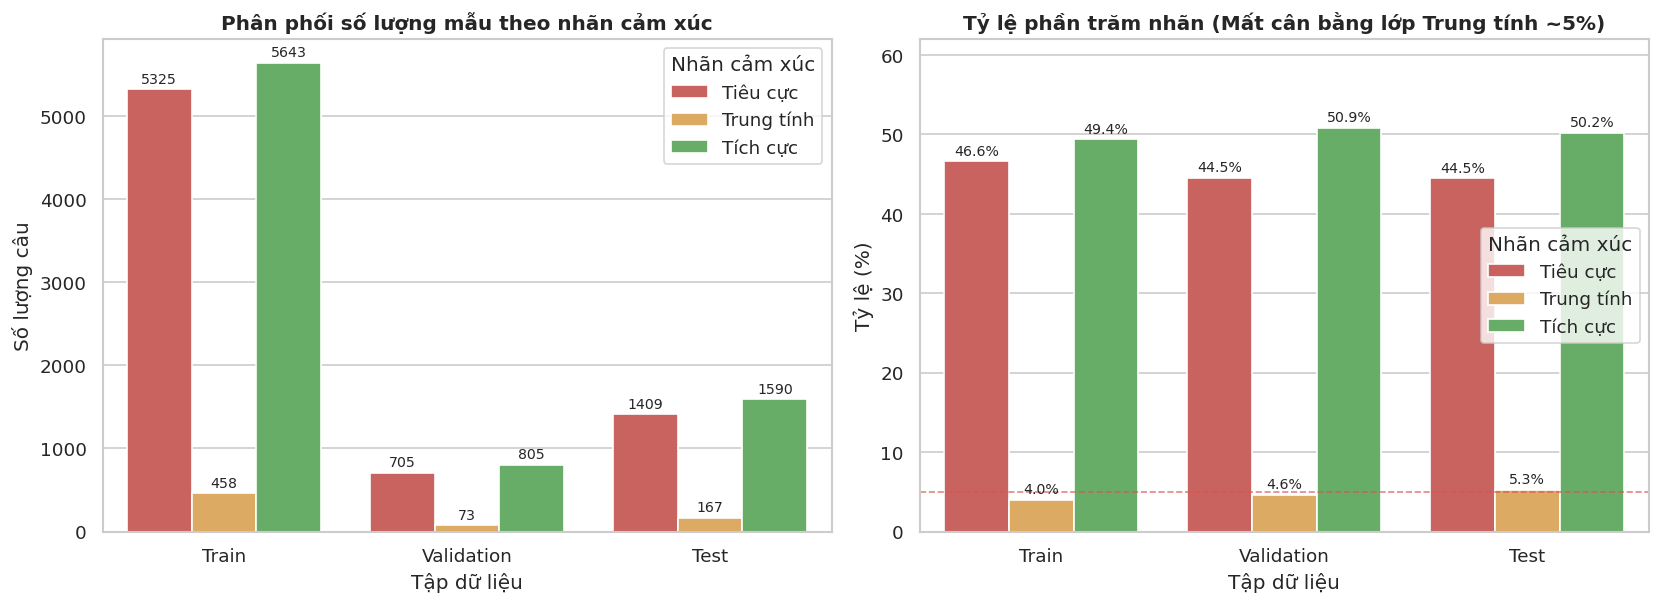
\includegraphics[width=0.95\textwidth]{figures/label_distribution.png}
    \caption{Phân phối số lượng và tỷ lệ phần trăm các nhãn cảm xúc trên UIT-VSFC (lớp Trung tính chỉ chiếm khoảng 4--5\%)}
    \label{fig:text_label_dist}
\end{figure}

\subsection{Phân phối độ dài câu}
Bảng~\ref{tab:text_length_stats} và Hình~\ref{fig:text_length_dist} thống kê độ dài câu theo số từ (tách bằng khoảng trắng) và số ký tự. Độ dài trung bình trên cả 3 tập dao động quanh 13,67--14,31 từ (trung vị 11 từ) và 56,36--59,08 ký tự. Phân vị thứ 95 (\texttt{P95}) là 31--34 từ và phân vị thứ 99 (\texttt{P99}) là 46--52,3 từ, trong khi câu dài nhất lên tới 161 từ. Vì trên 99\% câu có độ dài dưới 55 từ, việc chọn ngưỡng \texttt{max\_length=128} token cho mô hình PhoBERT vừa đảm bảo bao phủ gần như toàn vẹn ngữ cảnh câu, vừa tối ưu tốc độ và bộ nhớ GPU.

\begin{table}[htbp]
\centering
\caption{Thống kê phân phối độ dài câu theo số từ và số ký tự trên 3 tập}
\label{tab:text_length_stats}
\small
\resizebox{\textwidth}{!}{%
\begin{tabular}{|l|l|r|r|r|r|r|r|r|}
\hline
\textbf{Tập} & \textbf{Đơn vị} & \textbf{Mean} & \textbf{Std} & \textbf{Min} & \textbf{Median} & \textbf{P95} & \textbf{P99} & \textbf{Max} \\
\hline
Train      & Số từ    & 14,31 & 10,09 & 2 & 11,0 & 33,0  & 52,0  & 159 \\
Train      & Số ký tự & 59,08 & 43,08 & 4 & 47,0 & 141,0 & 218,8 & 660 \\
\hline
Validation & Số từ    & 13,67 & 9,91  & 2 & 11,0 & 31,0  & 46,0  & 161 \\
Validation & Số ký tự & 56,36 & 42,75 & 4 & 45,0 & 132,0 & 196,2 & 718 \\
\hline
Test       & Số từ    & 14,22 & 10,24 & 2 & 11,0 & 34,0  & 52,3  & 98  \\
Test       & Số ký tự & 58,84 & 44,12 & 4 & 46,0 & 147,0 & 221,3 & 411 \\
\hline
\end{tabular}%
}
\end{table}

\begin{figure}[htbp]
    \centering
    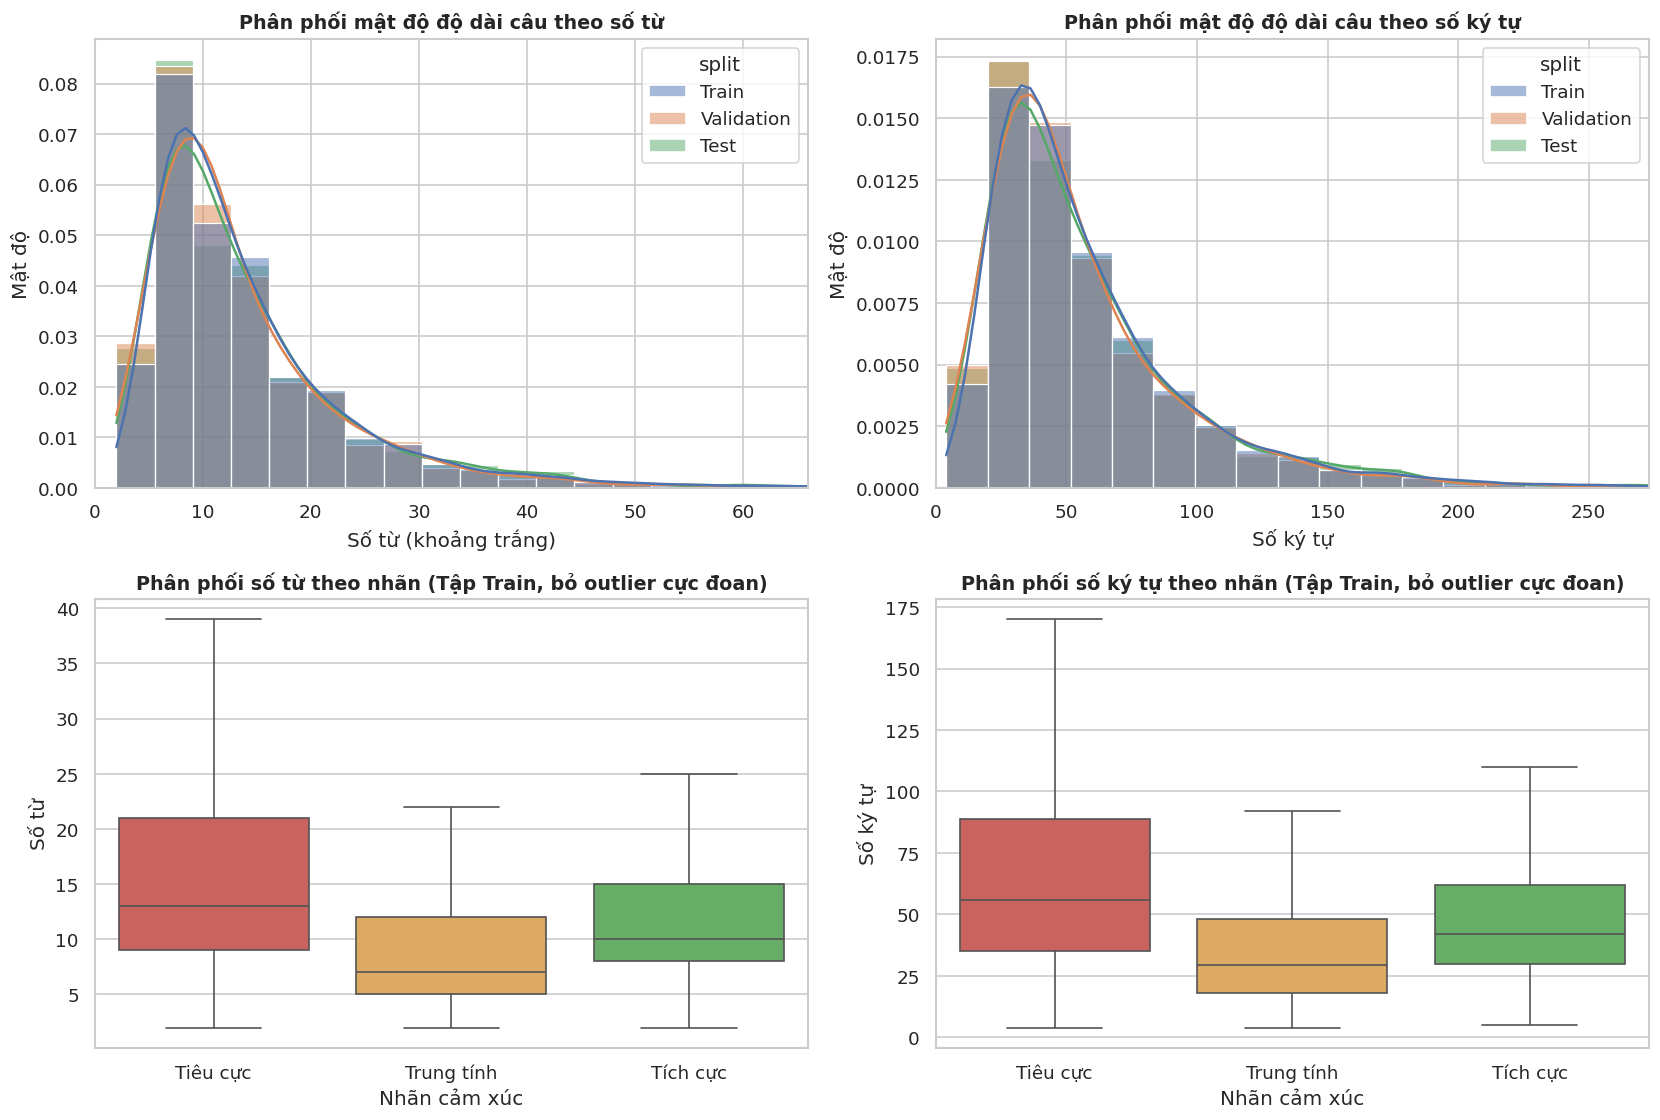
\includegraphics[width=0.95\textwidth]{figures/length_distribution.png}
    \caption{Phân phối mật độ và boxplot độ dài câu theo số từ và số ký tự}
    \label{fig:text_length_dist}
\end{figure}

\subsection{Tần suất token đặc thù và phân tích N-gram theo nhãn}
Trong phiên bản chuẩn hóa công khai của UIT-VSFC, tên riêng giảng viên/môn học đã được ẩn danh thành mã \texttt{wzjwz*} (ví dụ \texttt{wzjwz287}) và một số ký hiệu toán học/dấu câu được mã hóa thành \texttt{dot}, \texttt{fraction}, \texttt{colon}, \texttt{doublespace}. Kết quả kiểm tra tần suất trong Bảng~\ref{tab:text_special_tokens} và Hình~\ref{fig:text_special_tokens} cho thấy mã \texttt{wzjwz*} xuất hiện 237 lần (trên 210 câu, chiếm 1,84\%) ở tập \texttt{Train}, 20 lần ở tập \texttt{Validation} (1,14\%) và 76 lần (trên 73 câu, chiếm 2,31\%) ở tập \texttt{Test}; ngoài ra còn có \texttt{dot} (18 lần trên \texttt{Train}) và \texttt{fraction} (19 lần trên \texttt{Train}, 3 lần trên \texttt{Val}, 11 lần trên \texttt{Test}). Các token kỹ thuật này không mang ý nghĩa cảm xúc nên cần được lọc sạch ở bước tiền xử lý.

\begin{table}[htbp]
\centering
\caption{Tần suất xuất hiện các token đặc thù trong tập dữ liệu UIT-VSFC}
\label{tab:text_special_tokens}
\small
\begin{tabular}{|l|l|r|r|r|}
\hline
\textbf{Tập dữ liệu} & \textbf{Token đặc thù} & \textbf{Số lần xuất hiện} & \textbf{Số câu chứa token} & \textbf{Tỷ lệ câu (\%)} \\
\hline
Train      & \texttt{dot}      & 18  & 16  & 0,14\% \\
Train      & \texttt{fraction} & 19  & 18  & 0,16\% \\
Train      & \texttt{wzjwz*}   & 237 & 210 & 1,84\% \\
\hline
Validation & \texttt{fraction} & 3   & 3   & 0,19\% \\
Validation & \texttt{wzjwz*}   & 20  & 18  & 1,14\% \\
\hline
Test       & \texttt{fraction} & 11  & 10  & 0,32\% \\
Test       & \texttt{wzjwz*}   & 76  & 73  & 2,31\% \\
\hline
\end{tabular}
\end{table}

\begin{figure}[htbp]
    \centering
    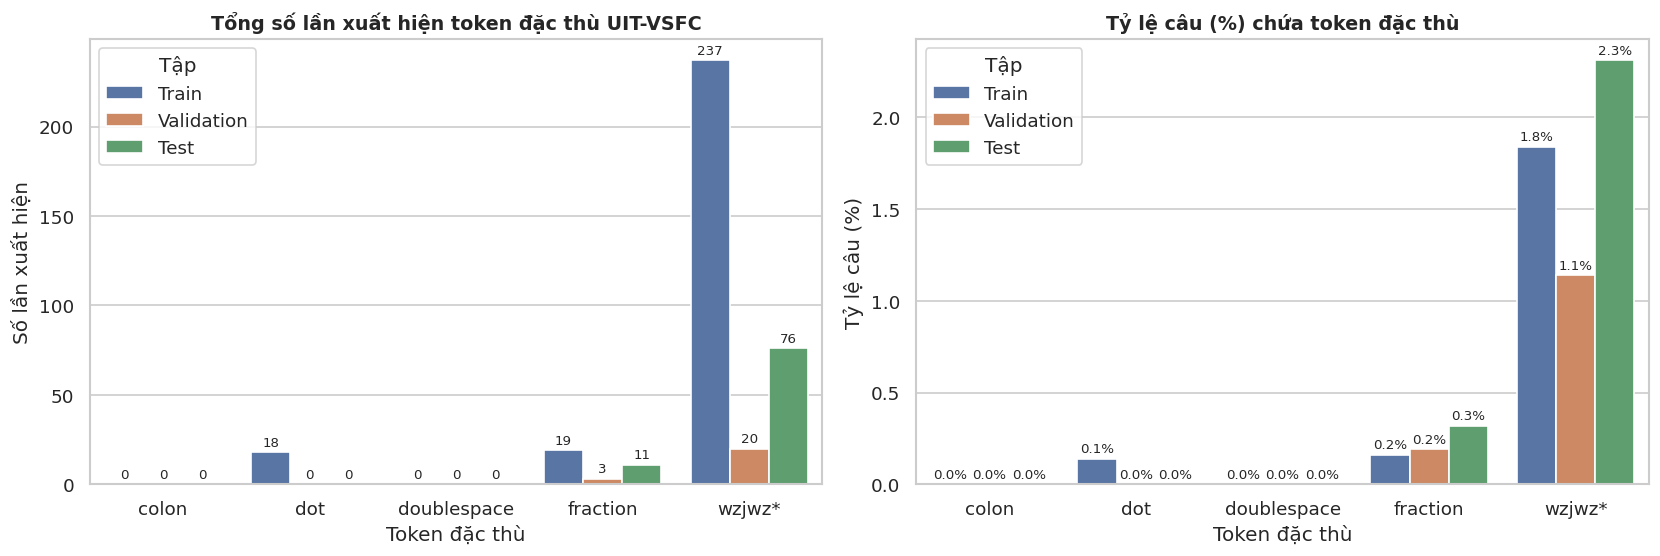
\includegraphics[width=0.92\textwidth]{figures/special_tokens_frequency.png}
    \caption{Tần suất xuất hiện và tỷ lệ câu chứa các token đặc thù của UIT-VSFC}
    \label{fig:text_special_tokens}
\end{figure}

Quan sát Top 15 Unigram và Bigram phổ biến nhất theo từng nhãn trên tập \texttt{Train} (Hình~\ref{fig:text_top_unigrams} và Hình~\ref{fig:text_top_bigrams}) cho thấy sự phân hóa từ vựng rõ rệt:
\begin{itemize}
    \item \textbf{Nhãn Tích cực:} Nổi bật với các từ/cụm từ biểu đạt sự hài lòng như \textit{``nhiệt tình''} (1.764 lần), \textit{``dễ hiểu''} (953 lần), \textit{``tận tâm''} (539 lần), \textit{``truyền đạt''} (321 lần), \textit{``rất''} (1.607 lần).
    \item \textbf{Nhãn Tiêu cực:} Tập trung quanh các chủ đề phàn nàn về \textit{``thực hành''} (721 lần), \textit{``bài tập''} (628 lần), \textit{``thời gian''} (322 lần), \textit{``lý thuyết''} (293 lần), \textit{``khó hiểu''} (246 lần), \textit{``đồ án''} (190 lần), và tần suất cao của từ phủ định \textit{``không''} (1.814 lần).
    \item \textbf{Nhãn Trung tính:} Đáng chú ý nhất là cụm \textit{``không có''} (52 lần) và \textit{``ý kiến''} (29 lần), \textit{``em không''} (20 lần) xuất hiện trong các phản hồi ngắn như \textit{``em không có ý kiến''}. Ngoài ra, nhiều câu trung tính cũng chứa các bigram như \textit{``thực hành''}, \textit{``bài tập''}, \textit{``hài lòng''}, tạo ra vùng chồng lấp từ vựng trực tiếp với hai lớp cực tính còn lại.
\end{itemize}

\begin{figure}[htbp]
    \centering
    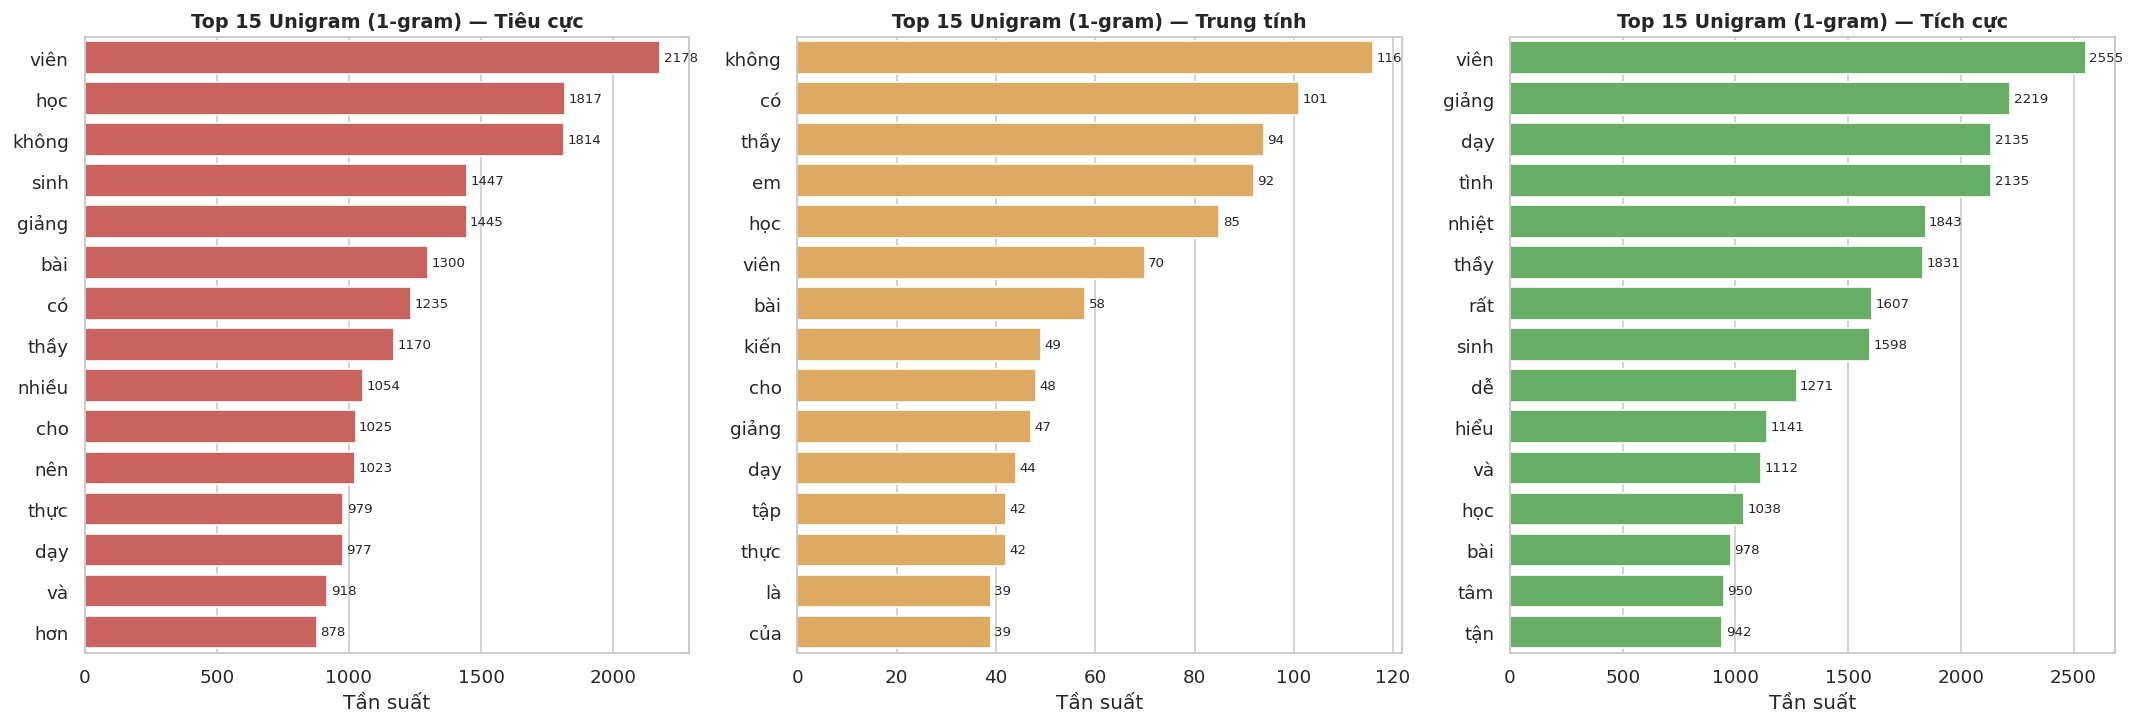
\includegraphics[width=0.98\textwidth]{figures/top_unigrams_by_label.png}
    \caption{Top 15 Unigram phổ biến nhất theo từng nhãn cảm xúc trên tập Train}
    \label{fig:text_top_unigrams}
\end{figure}

\begin{figure}[htbp]
    \centering
    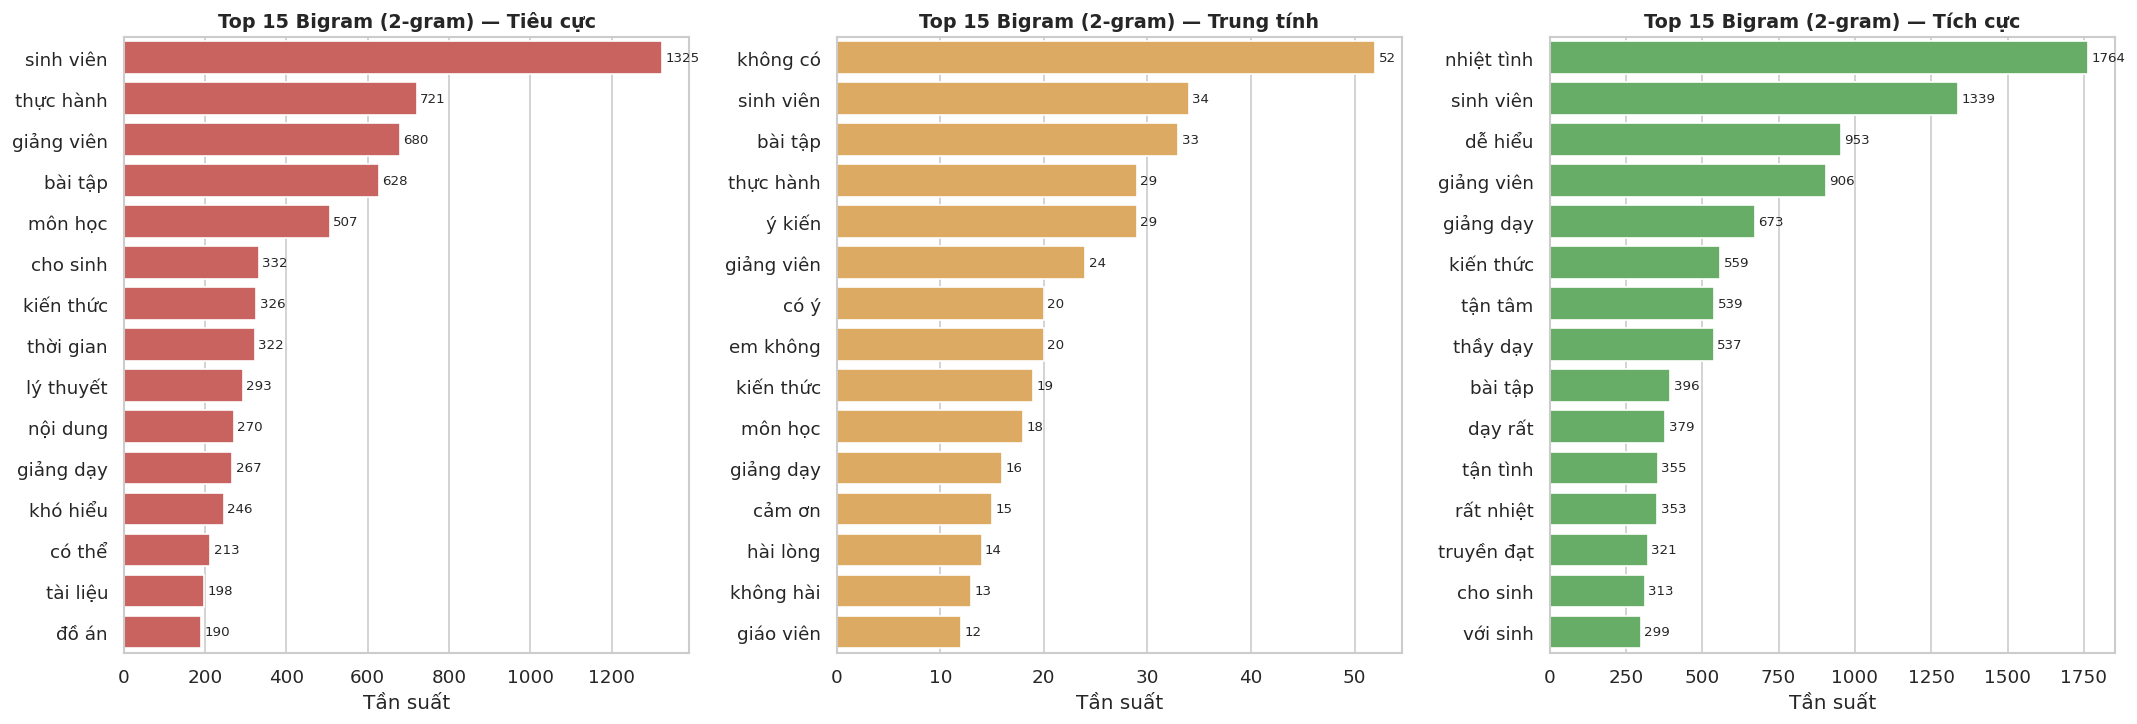
\includegraphics[width=0.98\textwidth]{figures/top_bigrams_by_label.png}
    \caption{Top 15 Bigram phổ biến nhất theo từng nhãn cảm xúc trên tập Train}
    \label{fig:text_top_bigrams}
\end{figure}

% ==============================================================================
\section{Thiết kế và kiến trúc Pipeline}

Để đáp ứng yêu cầu linh hoạt cấu hình và so sánh toàn diện giữa hướng tiếp cận truyền thống và hiện đại, hệ thống được module hóa thành các thành phần độc lập trong thư mục \texttt{modules/} và điều phối qua Google Colab Notebook (\texttt{Runtime -> Run all}, cố định hạt giống ngẫu nhiên \texttt{seed=42}).

\subsection{Module tiền xử lý cấu hình được (\texttt{VietnameseTextPreprocessor})}
Lớp \texttt{VietnameseTextPreprocessor} kế thừa \texttt{BaseEstimator} và \texttt{TransformerMixin} của \texttt{scikit-learn}, cho phép bật/tắt độc lập 5 bước:
\begin{enumerate}
    \item \texttt{lowercase}: Chuyển toàn bộ chuỗi về chữ thường (bật cho nhánh ML truyền thống; tắt cho PhoBERT để giữ thông tin chữ hoa).
    \item \texttt{clean\_special\_tokens}: Loại bỏ các token kỹ thuật \texttt{colon}, \texttt{dot}, \texttt{doublespace}, \texttt{fraction} và mã ẩn danh \texttt{wzjwz\textbackslash d*} bằng biểu thức chính quy.
    \item \texttt{remove\_punctuation}: Loại bỏ dấu câu ASCII và dấu câu tiếng Việt mở rộng (\texttt{“ ” ‘ ’ … – —}).
    \item \texttt{word\_segment}: Tách từ ghép tiếng Việt bằng \texttt{pyvi.ViTokenizer.tokenize} (ví dụ \textit{``giảng viên''} $\rightarrow$ \textit{``giảng\_viên''}).
    \item \texttt{remove\_stopwords}: Lọc các từ dừng tiếng Việt phổ thông nhưng \textbf{bắt buộc giữ lại danh sách trắng} gồm các từ phủ định, từ chuyển ý và phó từ mức độ (\textit{không, chưa, chẳng, chả, đừng, nhưng, tuy, hơi, quá, rất, lắm, cực\_kỳ, kém, thường\dots}) để không làm đảo ngược ngữ nghĩa cảm xúc.
\end{enumerate}

\subsection{Hai nhánh trích xuất đặc trưng}
\begin{itemize}
    \item \textbf{Nhánh 1 — Đặc trưng truyền thống (BoW \& TF-IDF):} Sử dụng \texttt{CountVectorizer} (\texttt{BoW (1,1)}, \texttt{max\_features=15.000}) và \texttt{TfidfVectorizer} (\texttt{sublinear\_tf=True}, \texttt{min\_df=2}) với hai cấu hình n-gram: Unigram \texttt{TF-IDF (1,1)} (\texttt{max\_features=15.000}) và Unigram + Bigram \texttt{TF-IDF (1,2)} (\texttt{max\_features=20.000}).
    \item \textbf{Nhánh 2 — Đặc trưng ngữ nghĩa học sâu (PhoBERT \texttt{.npy}):} Văn bản chỉ qua làm sạch token đặc thù và tách từ bằng \texttt{pyvi} (giữ nguyên chữ hoa và dấu câu), sau đó đưa qua mô hình tiền huấn luyện tiếng Việt \texttt{vinai/phobert-base-v2} trên GPU Tesla T4 với chế độ hỗn hợp độ chính xác FP16 (\texttt{autocast}, \texttt{batch\_size=64}, \texttt{max\_length=128}). Vector biểu diễn câu 768 chiều được rút trích bằng phép \textbf{Mean Pooling} có trọng số \texttt{attention\_mask} trên \texttt{last\_hidden\_state}:
    \[
        \mathbf{e} = \frac{\sum_{t=1}^{L} m_t \mathbf{h}_t}{\max\left(\sum_{t=1}^{L} m_t, 10^{-9}\right)} \in \mathbb{R}^{768}
    \]
    Kết quả được lưu xuống đĩa ở định dạng \texttt{float32} tại \texttt{features/phobert\_train.npy} $(11.426 \times 768)$, \texttt{features/phobert\_val.npy} $(1.583 \times 768)$ và \texttt{features/phobert\_test.npy} $(3.166 \times 768)$, sau đó nạp trực tiếp qua hàm \texttt{load\_embeddings()} để huấn luyện các mô hình phân loại.
\end{itemize}

\subsection{Ba nhóm mô hình phân loại và chiến lược xử lý mất cân bằng}
\begin{enumerate}
    \item \textbf{Pipeline 1 — Học máy truyền thống:} Đánh giá 3 thuật toán \texttt{MultinomialNB} ($\alpha=1{,}0$), \texttt{LogisticRegression} ($C=1{,}0$, \texttt{max\_iter=1000}) và \texttt{LinearSVC} ($C=1{,}0$, \texttt{max\_iter=2000}) trên các ma trận BoW/TF-IDF, so sánh trực tiếp giữa hai chế độ không cân bằng (\texttt{cw=none}) và cân bằng trọng số lớp (\texttt{cw=balanced}; riêng MultinomialNB sử dụng \texttt{compute\_sample\_weight}).
    \item \textbf{Pipeline 2 — Mô hình Lai (Hybrid trên PhoBERT \texttt{.npy}):} Các vector 768 chiều được chuẩn hóa qua \texttt{StandardScaler} trước khi đưa vào \texttt{LogisticRegression} ($C=0{,}5$), \texttt{LinearSVC} ($C=0{,}1$) và mạng nơ-ron đa tầng \texttt{MLPClassifier} gồm 2 tầng ẩn $(256, 64)$, hàm kích hoạt ReLU, \texttt{alpha=1e-3}, \texttt{early\_stopping=True}.
    \item \textbf{Pipeline 3 — Học sâu End-to-End Fine-tuning (Mở rộng điểm cộng):} Tinh chỉnh toàn bộ tham số của \texttt{vinai/phobert-base-v2} gắn đầu phân loại 3 lớp trong 3 epochs (\texttt{batch\_size=32}, \texttt{AdamW} với \texttt{lr=2e-5}, \texttt{weight\_decay=0,01}, lịch học Linear Warmup 10\% tổng số bước và gradient clipping $= 1{,}0$). Để cải thiện lớp thiểu số \textit{Trung tính} mà không gây quá nhiều dự đoán dương giả, hàm mất mát \texttt{CrossEntropyLoss} sử dụng trọng số lớp làm dịu theo căn bậc hai: $w'_c = \sqrt{w_c^{\text{balanced}}}$. Checkpoint tốt nhất được lựa chọn tự động dựa trên \textbf{Validation Macro F1}.
\end{enumerate}

% ==============================================================================
\section{Kết quả thực nghiệm và phân tích so sánh}

\subsection{Thí nghiệm 1: Khảo sát ảnh hưởng của tiền xử lý (Ablation Study)}
Bốn cấu hình tiền xử lý kết hợp bật/tắt tách từ (\texttt{WordSeg} vs \texttt{NoSeg}) và giữ/loại bỏ stopwords (\texttt{KeepSW} vs \texttt{RemoveSW}) được thử nghiệm trên đặc trưng cố định \texttt{TF-IDF (1,2)} với cả 3 bộ phân loại (\texttt{cw=balanced}). Bảng~\ref{tab:text_exp1} trình bày toàn bộ kết quả thu được.

\begin{table}[htbp]
\centering
\caption{Kết quả Thí nghiệm 1 — Khảo sát cấu hình tiền xử lý trên TF-IDF (1,2)}
\label{tab:text_exp1}
\scriptsize
\setlength{\tabcolsep}{4pt}
\resizebox{\textwidth}{!}{%
\begin{tabular}{|l|l|c|c|c|c|c|}
\hline
\textbf{Cấu hình tiền xử lý} & \textbf{Mô hình} & \textbf{Val Macro F1} & \textbf{Test Acc} & \textbf{Macro F1} & \textbf{Weighted F1} & \textbf{F1 (TT)} \\
\hline
C1: NoSeg + KeepSW   & LinearSVC          & \textbf{0,7714} & 0,8929 & 0,7293 & 0,8880 & 0,3525 \\
C1: NoSeg + KeepSW   & LogisticRegression & 0,7523 & 0,8654 & 0,7149 & 0,8710 & 0,3452 \\
C1: NoSeg + KeepSW   & MultinomialNB      & 0,7168 & 0,8253 & 0,6745 & 0,8355 & 0,2941 \\
\hline
C2: NoSeg + RemoveSW & LinearSVC          & 0,7342 & 0,8765 & 0,7140 & 0,8727 & 0,3379 \\
C2: NoSeg + RemoveSW & LogisticRegression & 0,7197 & 0,8380 & 0,6870 & 0,8484 & 0,3056 \\
C2: NoSeg + RemoveSW & MultinomialNB      & 0,6863 & 0,8048 & 0,6529 & 0,8188 & 0,2620 \\
\hline
C3: WordSeg + KeepSW & LinearSVC          & 0,7681 & \textbf{0,8945} & \textbf{0,7359} & \textbf{0,8900} & \textbf{0,3701} \\
C3: WordSeg + KeepSW & LogisticRegression & 0,7535 & 0,8705 & 0,7207 & 0,8756 & 0,3538 \\
C3: WordSeg + KeepSW & MultinomialNB      & 0,7332 & 0,8402 & 0,6916 & 0,8520 & 0,3124 \\
\hline
C4: WordSeg + RemoveSW & LinearSVC        & 0,7305 & 0,8677 & 0,7042 & 0,8657 & 0,3215 \\
C4: WordSeg + RemoveSW & LogisticRegression & 0,7136 & 0,8427 & 0,6931 & 0,8538 & 0,3135 \\
C4: WordSeg + RemoveSW & MultinomialNB    & 0,6978 & 0,8130 & 0,6601 & 0,8284 & 0,2632 \\
\hline
\end{tabular}%
}
\end{table}

Từ Bảng~\ref{tab:text_exp1}, có thể rút ra hai nhận xét quan trọng:
\begin{enumerate}
    \item \textbf{Loại bỏ stopwords làm giảm hiệu năng đáng kể:} Ngay cả khi đã giữ lại danh sách trắng các từ phủ định, việc xóa stopwords (\texttt{C2}, \texttt{C4}) khiến Macro F1 giảm khoảng 1,5--3,2 điểm phần trăm so với giữ nguyên (\texttt{C1}, \texttt{C3}). Nguyên nhân là nhiều câu phản hồi sinh viên rất ngắn (trung vị 11 từ) và đặc biệt ở lớp \textit{Trung tính} các từ nối như \textit{``có''}, \textit{``của''}, \textit{``là''}, \textit{``em''} góp phần hình thành cụm đặc trưng (ví dụ \textit{``em không có ý kiến''}).
    \item \textbf{Tách từ tiếng Việt giúp ổn định kết quả trên tập Test:} Với \texttt{TF-IDF (1,2)}, cấu hình \texttt{C3 (WordSeg + KeepSW)} đạt Test Macro F1 cao nhất trong Thí nghiệm 1 (\textbf{0,7359}) và F1 lớp Trung tính đạt \textbf{0,3701}, trong khi trên tập Validation cấu hình \texttt{C1 (NoSeg + KeepSW)} nhỉnh hơn đôi chút (0,7714 so với 0,7681) nên được chọn tự động làm đầu vào cho Thí nghiệm 2 nhằm tuân thủ nguyên tắc không dùng tập Test để chọn siêu tham số.
\end{enumerate}

\subsection{Thí nghiệm 2: Pipeline Học máy truyền thống}
Bảng~\ref{tab:text_exp2} tổng hợp toàn bộ 18 cấu hình của Pipeline truyền thống trên 3 kiểu biểu diễn (\texttt{BoW (1,1)}, \texttt{TF-IDF (1,1)}, \texttt{TF-IDF (1,2)}) kết hợp 3 mô hình và hai chế độ trọng số lớp.

\begin{table}[htbp]
\centering
\caption{Kết quả Thí nghiệm 2 — Pipeline Học máy truyền thống (18 cấu hình, sắp xếp theo Test Macro F1)}
\label{tab:text_exp2}
\scriptsize
\setlength{\tabcolsep}{3.5pt}
\resizebox{\textwidth}{!}{%
\begin{tabular}{|l|c|c|c|c|c|c|c|}
\hline
\textbf{Cấu hình mô hình} & \textbf{Val MF1} & \textbf{Acc} & \textbf{Macro P} & \textbf{Macro R} & \textbf{Macro F1} & \textbf{F1 (TC)} & \textbf{F1 (TT)} \\
\hline
TF-IDF (1,1) + LinearSVC (cw=balanced)          & 0,7619 & 0,8759 & 0,7331 & 0,7534 & \textbf{0,7417} & 0,8967 & \textbf{0,4173} \\
BoW (1,1) + LinearSVC (cw=balanced)             & 0,7514 & 0,8702 & 0,7279 & 0,7468 & 0,7362 & 0,8866 & 0,4130 \\
TF-IDF (1,2) + LinearSVC (cw=balanced)          & \textbf{0,7714} & 0,8929 & 0,7531 & 0,7161 & 0,7293 & 0,9143 & 0,3525 \\
TF-IDF (1,2) + LogisticRegression (cw=balanced) & 0,7523 & 0,8654 & 0,7063 & 0,7306 & 0,7149 & 0,8905 & 0,3452 \\
BoW (1,1) + LogisticRegression (cw=balanced)    & 0,7395 & 0,8468 & 0,7011 & 0,7604 & 0,7143 & 0,8710 & 0,3683 \\
BoW (1,1) + LogisticRegression (cw=none)        & 0,7437 & 0,8850 & 0,7711 & 0,6922 & 0,7125 & 0,9020 & 0,3237 \\
BoW (1,1) + LinearSVC (cw=none)                 & 0,7275 & 0,8806 & 0,7621 & 0,6923 & 0,7120 & 0,8976 & 0,3306 \\
TF-IDF (1,1) + LogisticRegression (cw=balanced) & 0,7146 & 0,8377 & 0,6971 & \textbf{0,7649} & 0,7085 & 0,8643 & 0,3620 \\
TF-IDF (1,2) + LinearSVC (cw=none)              & 0,7530 & \textbf{0,8964} & 0,8085 & 0,6848 & 0,7050 & 0,9138 & 0,2791 \\
TF-IDF (1,1) + LinearSVC (cw=none)              & 0,7088 & 0,8850 & 0,7917 & 0,6785 & 0,6987 & 0,9032 & 0,2831 \\
TF-IDF (1,2) + MultinomialNB (cw=balanced)      & 0,7168 & 0,8253 & 0,6662 & 0,6964 & 0,6745 & 0,8473 & 0,2941 \\
TF-IDF (1,1) + LogisticRegression (cw=none)     & 0,7019 & 0,8819 & 0,7922 & 0,6464 & 0,6521 & 0,8987 & 0,1474 \\
BoW (1,1) + MultinomialNB (cw=balanced)         & 0,6759 & 0,7963 & 0,6451 & 0,6821 & 0,6514 & 0,8120 & 0,2744 \\
TF-IDF (1,2) + LogisticRegression (cw=none)     & 0,6898 & 0,8898 & \textbf{0,8235} & 0,6470 & 0,6484 & 0,9061 & 0,1202 \\
TF-IDF (1,1) + MultinomialNB (cw=balanced)      & 0,6832 & 0,7887 & 0,6426 & 0,6826 & 0,6473 & 0,8081 & 0,2722 \\
BoW (1,1) + MultinomialNB (cw=none)             & 0,6647 & 0,8304 & 0,6457 & 0,6207 & 0,6252 & 0,8443 & 0,1606 \\
TF-IDF (1,2) + MultinomialNB (cw=none)          & 0,5960 & 0,8575 & 0,5724 & 0,6047 & 0,5872 & 0,8719 & 0,0000 \\
TF-IDF (1,1) + MultinomialNB (cw=none)          & 0,5867 & 0,8392 & 0,5613 & 0,5922 & 0,5747 & 0,8525 & 0,0000 \\
\hline
\end{tabular}%
}
\end{table}

Phân tích Thí nghiệm 2 cho thấy tác động rõ rệt của chiến lược xử lý mất cân bằng dữ liệu:
\begin{itemize}
    \item Khi không dùng \texttt{class\_weight} (\texttt{cw=none}), \texttt{TF-IDF + MultinomialNB} đạt F1 lớp \textit{Trung tính} bằng \textbf{0,0000} (bỏ qua hoàn toàn lớp thiểu số do xác suất tiên nghiệm quá nhỏ), còn \texttt{TF-IDF (1,2) + LogisticRegression} chỉ đạt F1 (Trung tính) $= 0{,}1202$ dù Accuracy vẫn ở mức $88{,}98\%$.
    \item Khi bật \texttt{class\_weight='balanced'}, Macro F1 của tất cả mô hình đều tăng mạnh: \texttt{TF-IDF (1,1) + LinearSVC (cw=balanced)} vươn lên dẫn đầu nhóm ML truyền thống với \textbf{Macro F1 = 0,7417} (Accuracy 87,59\%, Weighted F1 = 0,8787), đẩy F1 lớp \textit{Trung tính} từ 0,2831 lên \textbf{0,4173} (Precision 0,3812; Recall 0,4611; trong khi lớp Tiêu cực đạt F1 = 0,8967 và lớp Tích cực đạt F1 = 0,9112).
    \item Trong nhóm không cân bằng, \texttt{TF-IDF (1,2) + LinearSVC (cw=none)} đạt Accuracy cao nhất nhóm truyền thống (89,64\%) nhưng đánh đổi bằng Macro F1 thấp hơn (0,7050).
\end{itemize}

\subsection{Thí nghiệm 3: Pipeline Lai trên đặc trưng PhoBERT (\texttt{.npy})}
Sau khi trích xuất và lưu 3 tệp embedding \texttt{features/phobert\_*.npy} kích thước 768 chiều, các bộ phân loại tuyến tính và mạng nơ-ron MLP được huấn luyện trực tiếp trên các tệp này. Bảng~\ref{tab:text_exp3} cho thấy biểu diễn ngữ nghĩa từ PhoBERT giúp vượt xa toàn bộ các mô hình đếm từ truyền thống ngay cả khi vector đặc trưng bị đóng băng.

\begin{table}[htbp]
\centering
\caption{Kết quả Thí nghiệm 3 — Pipeline Lai sử dụng PhoBERT Embeddings (\texttt{.npy})}
\label{tab:text_exp3}
\scriptsize
\setlength{\tabcolsep}{4pt}
\resizebox{\textwidth}{!}{%
\begin{tabular}{|l|c|c|c|c|c|c|c|}
\hline
\textbf{Mô hình trên PhoBERT \texttt{.npy}} & \textbf{Val MF1} & \textbf{Acc} & \textbf{Macro P} & \textbf{Macro R} & \textbf{Macro F1} & \textbf{F1 (TC)} & \textbf{F1 (TT)} \\
\hline
PhoBERT (.npy) + MLP (256-64)               & \textbf{0,7950} & \textbf{0,9157} & \textbf{0,8069} & 0,7511 & \textbf{0,7712} & \textbf{0,9345} & \textbf{0,4396} \\
PhoBERT (.npy) + LinearSVC (cw=balanced)    & 0,7688 & 0,8996 & 0,7593 & \textbf{0,7625} & 0,7609 & 0,9243 & 0,4307 \\
PhoBERT (.npy) + LinearSVC (cw=none)        & 0,7764 & 0,9078 & 0,7873 & 0,7418 & 0,7589 & 0,9312 & 0,4158 \\
PhoBERT (.npy) + LogisticRegression (none)  & 0,7824 & 0,8955 & 0,7623 & 0,7365 & 0,7474 & 0,9190 & 0,4027 \\
PhoBERT (.npy) + LogisticRegression (bal.)  & 0,7617 & 0,8863 & 0,7389 & 0,7565 & 0,7466 & 0,9124 & 0,4087 \\
\hline
\end{tabular}%
}
\end{table}

Mô hình tốt nhất nhóm Lai là \textbf{PhoBERT (.npy) + MLP (256-64)}, đạt \textbf{Accuracy = 91,57\%}, \textbf{Macro F1 = 0,7712} (tăng +2,95 điểm phần trăm so với mô hình ML truyền thống tốt nhất 0,7417), đồng thời F1 lớp \textit{Tiêu cực} đạt 0,9345, \textit{Tích cực} đạt 0,9394 và \textit{Trung tính} đạt 0,4396. Điều này chứng tỏ quan hệ phi tuyến của 2 tầng ẩn $(256, 64)$ khai thác thông tin ngữ cảnh trong không gian 768 chiều hiệu quả hơn siêu phẳng tuyến tính đơn thuần.

\subsection{Thí nghiệm 4 (Mở rộng): Fine-tuning End-to-End \texttt{vinai/phobert-base-v2}}
Quá trình tinh chỉnh trực tiếp toàn bộ mạng PhoBERT trong 3 epochs (với trọng số lớp căn bậc hai) được ghi nhận trong Bảng~\ref{tab:text_exp4_hist}. Mô hình hội tụ rất nhanh: ở Epoch 2, \texttt{Val Macro F1} đạt đỉnh \textbf{0,8766} (\texttt{Val Accuracy = 95,51\%}, \texttt{Val F1 Trung tính = 0,6977}) trước khi có dấu hiệu chững nhẹ ở Epoch 3 (0,8708). Do cơ chế chọn checkpoint tốt nhất theo Validation Macro F1, trọng số ở Epoch 2 được phục hồi để đánh giá trên tập Test.

\begin{table}[htbp]
\centering
\caption{Lịch sử huấn luyện PhoBERT Fine-tuning End-to-End qua 3 Epochs}
\label{tab:text_exp4_hist}
\small
\begin{tabular}{|c|c|c|c|c|}
\hline
\textbf{Epoch} & \textbf{Train Loss} & \textbf{Val Accuracy} & \textbf{Val Macro F1} & \textbf{Val F1 (Trung tính)} \\
\hline
1 & 0,4867 & 0,9457 & 0,8567 & 0,6557 \\
\hline
\textbf{2 (Best)} & \textbf{0,2487} & \textbf{0,9551} & \textbf{0,8766} & \textbf{0,6977} \\
\hline
3 & 0,1849 & 0,9514 & 0,8708 & 0,6866 \\
\hline
\end{tabular}
\end{table}

Trên tập Test độc lập (3.166 mẫu), \textbf{PhoBERT End-to-End Fine-tune (cw=sqrt-bal)} đạt bước nhảy vọt toàn diện (Bảng~\ref{tab:text_exp4_report}): \textbf{Accuracy = 93,68\%}, \textbf{Macro Precision = 0,8572}, \textbf{Macro Recall = 0,8122}, \textbf{Macro F1 = 0,8309} và \textbf{Weighted F1 = 0,9345}. Đặc biệt, lớp thiểu số \textit{Trung tính} đạt F1 = \textbf{0,5850} (tăng +16,77 điểm phần trăm so với ML truyền thống và +14,54 điểm phần trăm so với PhoBERT \texttt{.npy} đóng băng).

\begin{table}[htbp]
\centering
\caption{Báo cáo phân loại chi tiết trên tập Test của mô hình tốt nhất (PhoBERT End-to-End Fine-tune)}
\label{tab:text_exp4_report}
\small
\begin{tabular}{|l|c|c|c|r|}
\hline
\textbf{Nhãn cảm xúc} & \textbf{Precision} & \textbf{Recall} & \textbf{F1-score} & \textbf{Support} \\
\hline
Tiêu cực   & 0,9344 & 0,9702 & 0,9519 & 1.409 \\
Trung tính & 0,6772 & 0,5150 & 0,5850 & 167   \\
Tích cực   & 0,9600 & 0,9516 & 0,9558 & 1.590 \\
\hline
\textbf{Accuracy}     & \multicolumn{3}{c|}{\textbf{0,9368}} & 3.166 \\
\textbf{Macro avg}    & \textbf{0,8572} & \textbf{0,8122} & \textbf{0,8309} & 3.166 \\
\textbf{Weighted avg} & 0,9337 & 0,9368 & 0,9345 & 3.166 \\
\hline
\end{tabular}
\end{table}

\subsection{Tổng hợp so sánh và trực quan hóa Confusion Matrix}
Bảng~\ref{tab:text_summary_top} và Hình~\ref{fig:text_model_cmp} tóm tắt bảng xếp hạng các đại diện tiêu biểu từ 3 nhóm phương pháp. Sự thăng tiến đều đặn về Macro F1 ($0{,}7417 \rightarrow 0{,}7712 \rightarrow 0{,}8309$) và F1 lớp Trung tính ($0{,}4173 \rightarrow 0{,}4396 \rightarrow 0{,}5850$) khẳng định giá trị của việc biểu diễn ngữ cảnh sâu và tinh chỉnh đầu cuối.

\begin{table}[htbp]
\centering
\caption{So sánh các mô hình đại diện tốt nhất của từng nhóm phương pháp trên tập Test}
\label{tab:text_summary_top}
\scriptsize
\setlength{\tabcolsep}{4pt}
\resizebox{\textwidth}{!}{%
\begin{tabular}{|l|l|c|c|c|c|c|}
\hline
\textbf{Nhóm phương pháp} & \textbf{Mô hình đại diện} & \textbf{Acc} & \textbf{Macro F1} & \textbf{F1 (TC)} & \textbf{F1 (TT)} & \textbf{F1 (Tích cực)} \\
\hline
ML truyền thống   & TF-IDF (1,1) + LinearSVC (cw=balanced) & 0,8759 & 0,7417 & 0,8967 & 0,4173 & 0,9112 \\
Lai (PhoBERT .npy) & PhoBERT (.npy) + MLP (256-64)         & 0,9157 & 0,7712 & 0,9345 & 0,4396 & 0,9394 \\
Deep Learning E2E & PhoBERT Fine-tune (cw=sqrt-bal)        & \textbf{0,9368} & \textbf{0,8309} & \textbf{0,9519} & \textbf{0,5850} & \textbf{0,9558} \\
\hline
\end{tabular}%
}
\end{table}

\begin{figure}[htbp]
    \centering
    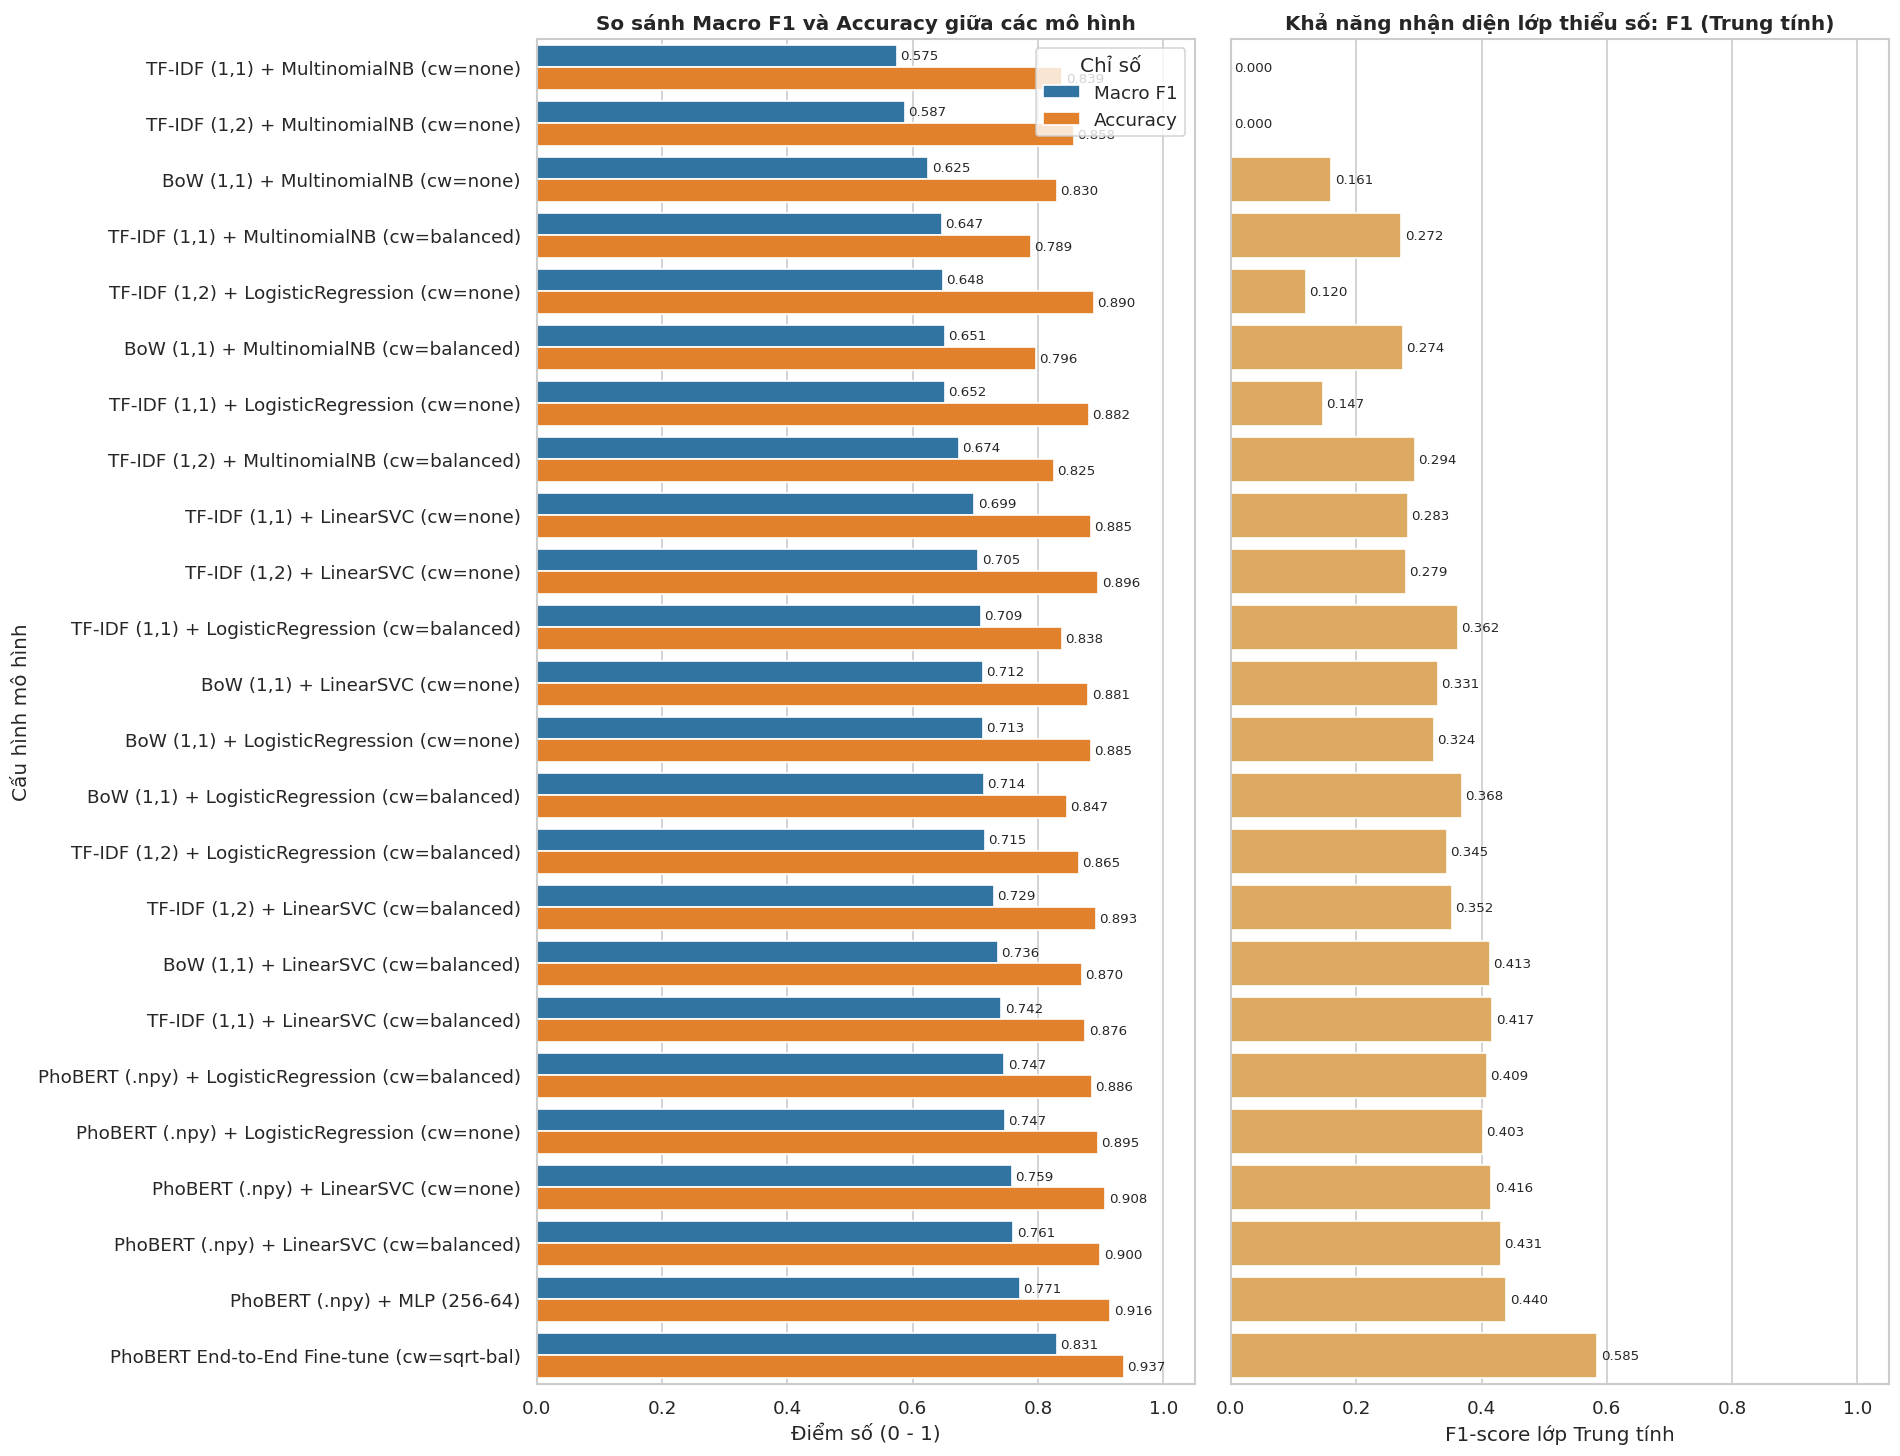
\includegraphics[width=0.98\textwidth]{figures/model_comparison.png}
    \caption{So sánh tổng hợp 24 cấu hình mô hình về Macro F1, Accuracy và F1 lớp Trung tính}
    \label{fig:text_model_cmp}
\end{figure}

Quan sát hai ma trận nhầm lẫn trong Hình~\ref{fig:text_cm_compare}:
\begin{itemize}
    \item Ở \textbf{TF-IDF (1,1) + LinearSVC (cw=balanced)}, độ nhạy trên hai lớp đa số đạt $90{,}8\%$ (1.280/1.409 câu Tiêu cực) và $89{,}1\%$ (1.416/1.590 câu Tích cực), nhưng vẫn còn 118 câu Tích cực (7,4\%) bị dự đoán nhầm thành Tiêu cực và 77/167 câu Trung tính (46,1\%) được nhận diện đúng.
    \item Ở \textbf{PhoBERT End-to-End Fine-tune}, tỷ lệ nhận diện đúng tăng mạnh trên cả 3 lớp: \textit{Tiêu cực} đạt \textbf{97,0\%} (1.367/1.409), \textit{Tích cực} đạt \textbf{95,2\%} (1.513/1.590) và \textit{Trung tính} đạt \textbf{51,5\%} (86/167). Sự nhầm lẫn giữa hai cực đối lập Tiêu cực--Tích cực giảm xuống rất thấp (chỉ 1,4\% và 3,6\%); phần lớn lỗi còn lại tập trung quanh ranh giới giữa lớp \textit{Trung tính} với hai lớp còn lại (22,8\% sang Tiêu cực và 25,7\% sang Tích cực).
\end{itemize}

\begin{figure}[htbp]
    \centering
    \begin{subfigure}[b]{0.48\textwidth}
        \centering
        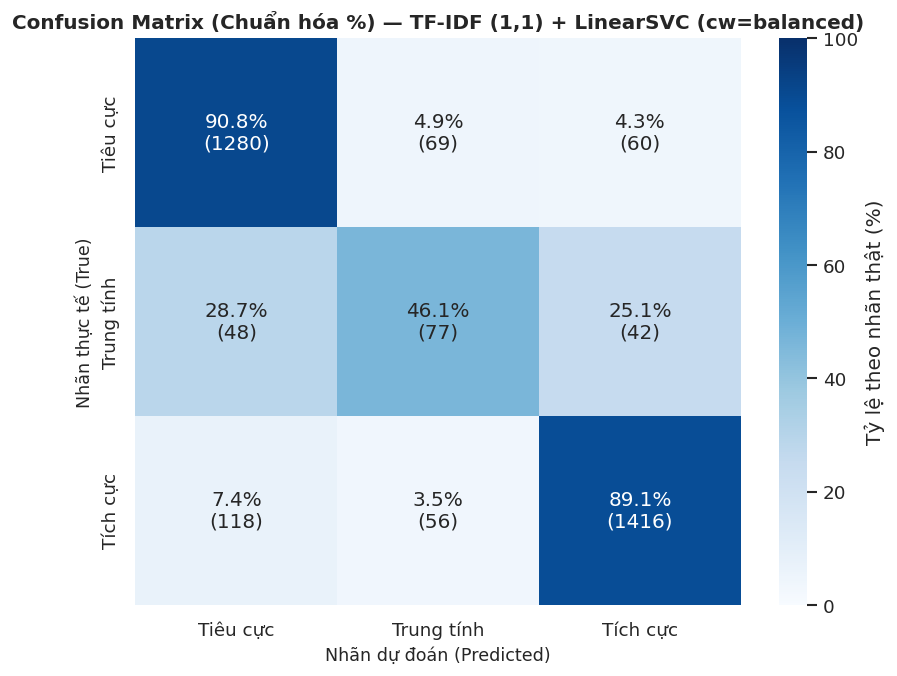
\includegraphics[width=\textwidth]{figures/confusion_matrix_traditional_best.png}
        \caption{ML truyền thống: TF-IDF (1,1) + LinearSVC}
    \end{subfigure}\hfill
    \begin{subfigure}[b]{0.48\textwidth}
        \centering
        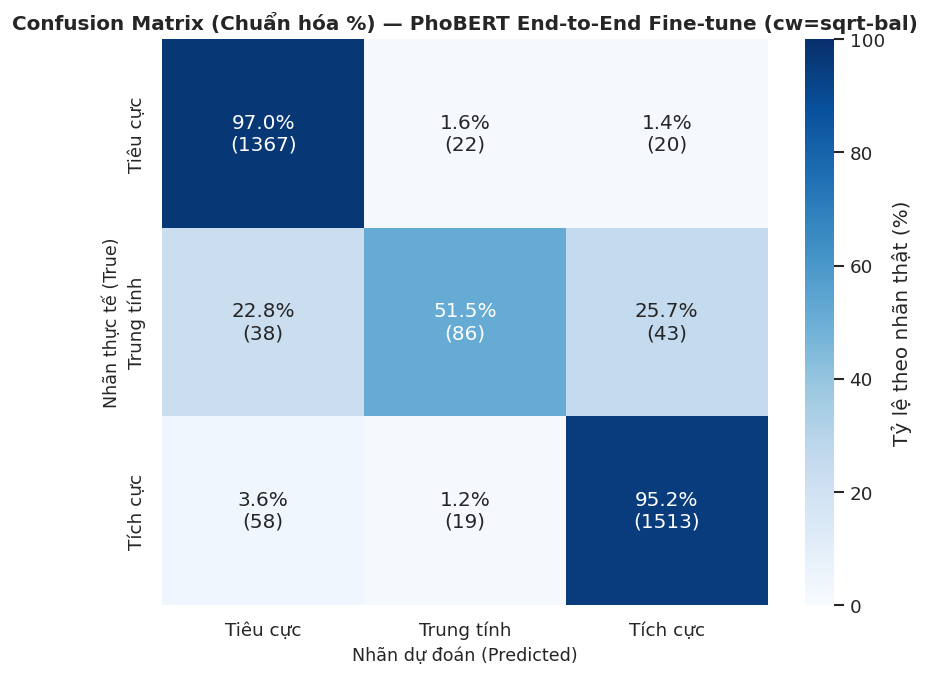
\includegraphics[width=\textwidth]{figures/confusion_matrix_best.png}
        \caption{Tốt nhất toàn cục: PhoBERT Fine-tune}
    \end{subfigure}
    \caption{Đối chiếu Confusion Matrix chuẩn hóa (\%) trên tập Test}
    \label{fig:text_cm_compare}
\end{figure}

% ==============================================================================
\section{Đánh giá ưu nhược điểm và phân tích lỗi (Error Analysis)}

\subsection{So sánh ưu điểm và hạn chế giữa các hướng tiếp cận}
\begin{itemize}
    \item \textbf{Pipeline ML truyền thống (BoW/TF-IDF + NB/LR/LinearSVC):} \textit{Ưu điểm:} Huấn luyện cực nhanh chỉ trong vài giây trên CPU, dung lượng gọn nhẹ, dễ kiểm tra trọng số từng từ khóa. \textit{Hạn chế:} Biểu diễn túi từ bỏ qua trật tự và ngữ cảnh câu dài, dễ nhầm khi gặp phủ định kép hoặc hàm ý mỉa mai; lớp Trung tính gần như bị lấn át nếu không cân bằng trọng số.
    \item \textbf{Pipeline Lai (PhoBERT \texttt{.npy} + LR/LinearSVC/MLP):} \textit{Ưu điểm:} Chỉ cần trích xuất embedding một lần và lưu thành file \texttt{.npy}, giúp thử nghiệm nhanh nhiều bộ phân loại trên không gian ngữ nghĩa 768 chiều, cải thiện rõ rệt cả Accuracy và Macro F1. \textit{Hạn chế:} Embedding bị đóng băng từ tác vụ tiền huấn luyện tổng quát nên chưa định hình riêng ranh giới phân tách cho lớp \textit{Trung tính} trong ngữ cảnh khảo sát sinh viên.
    \item \textbf{Pipeline Học sâu End-to-End (PhoBERT Fine-tuning):} \textit{Ưu điểm:} Tinh chỉnh toàn bộ tầng Transformer thích ứng trực tiếp với tập dữ liệu, đạt kết quả vượt trội trên mọi chỉ số (Macro F1 = 0,8309, giảm tổng số lỗi trên Test xuống còn \textbf{200/3.166 mẫu}, tương ứng tỷ lệ lỗi chỉ \textbf{6,32\%}). \textit{Hạn chế:} Đòi hỏi GPU khi huấn luyện/suy luận và kích thước mô hình lớn ($\sim 540$\,MB).
\end{itemize}

\subsection{Phân tích lỗi định tính (Error Analysis)}
Để hiểu rõ bản chất 200 mẫu dự đoán sai của mô hình tốt nhất (\textit{PhoBERT End-to-End Fine-tune}), Bảng~\ref{tab:text_error_analysis} trích xuất 15 mẫu đại diện phân bổ đều qua các cặp nhầm lẫn phổ biến:

\begin{table}[htbp]
\centering
\caption{15 mẫu dự đoán sai tiêu biểu của mô hình PhoBERT End-to-End Fine-tune trên tập Test}
\label{tab:text_error_analysis}
\scriptsize
\setlength{\tabcolsep}{3.5pt}
\begin{tabularx}{\textwidth}{|r|>{\raggedright\arraybackslash}X|l|l|c|p{3.0cm}|}
\hline
\textbf{ID} & \textbf{Văn bản gốc (tập Test)} & \textbf{Nhãn thật} & \textbf{Dự đoán} & \textbf{Tự tin} & \textbf{Nhóm nguyên nhân} \\
\hline
271  & \textit{`` các bạn có hiểu ý thầy wzjwz287 không ạ '' ( \dots} & Tiêu cực & Trung tính & 0,7754 & Trích dẫn lời nói gián tiếp \\
2705 & \textit{nâng cấp thiết bị phòng lab .} & Tiêu cực & Trung tính & 0,9424 & Đề xuất cải thiện hàm ý chê \\
2723 & \textit{em chưa bao giờ được thầy reply mail .} & Tiêu cực & Trung tính & 0,5353 & Câu tường thuật thiếu từ chê \\
1527 & \textit{nghiêm khắc trong khi dạy , kiến thức chuyên n\dots} & Tiêu cực & Tích cực & 0,9849 & Câu pha trộn hai vế đối lập \\
3015 & \textit{định hướng từ sớm về cách tiếp cận đồ án đối v\dots} & Tiêu cực & Tích cực & 0,8455 & Góp ý mang tính xây dựng \\
\hline
585  & \textit{em nghĩ như vậy sẽ tốt hơn vì họ sẽ biết được \dots} & Trung tính & Tiêu cực & 0,9745 & Đề xuất dài, ranh giới gán nhãn \\
1450 & \textit{thêm nhiều bài tập hay .} & Trung tính & Tiêu cực & 0,9736 & Đề xuất ``thêm bài tập'' \\
2337 & \textit{cho bài tập từ dễ tới khó .} & Trung tính & Tiêu cực & 0,9771 & Góp ý trung lập dễ hiểu nhầm \\
362  & \textit{cô cho em 10 điểm thực hành colonlove .} & Trung tính & Tích cực & 0,8707 & Nhiễu nhãn / biểu cảm tích cực \\
1447 & \textit{thầy dạy khá ổn .} & Trung tính & Tích cực & 0,9486 & Đánh giá tích cực nhẹ vs trung tính \\
\hline
1584 & \textit{môn học này rất hay và rất khó và rất đáng để \dots} & Tích cực & Tiêu cực & 0,6103 & Pha trộn từ \textit{``hay''} và \textit{``khó''} \\
1818 & \textit{được nói cặp .} & Tích cực & Tiêu cực & 0,7234 & Câu quá ngắn, thiếu ngữ cảnh \\
1987 & \textit{giảng viên dạy chậm , dễ tiếp thu .} & Tích cực & Tiêu cực & 0,9332 & Từ \textit{``dạy chậm''} thường là chê \\
1511 & \textit{không có điều gì không hài lòng .} & Tích cực & Trung tính & 0,9426 & Phủ định kép (\textit{không\dots không}) \\
2374 & \textit{hỗ trợ sinh viên làm đồ án .} & Tích cực & Trung tính & 0,6897 & Câu mô tả trung hòa thiếu tính từ \\
\hline
\end{tabularx}
\end{table}

Qua phân tích 15 mẫu trên, nguyên nhân lỗi tập trung vào 4 nhóm chính:
\begin{enumerate}
    \item \textbf{Ranh giới mờ giữa góp ý Trung tính và Tiêu cực/Tích cực:} Các câu đề xuất như \textit{``nâng cấp thiết bị phòng lab .''} (ID 2705) hay \textit{``thêm nhiều bài tập hay .''} (ID 1450) không có từ ngữ cảm xúc mạnh nhưng được người gán nhãn phân vào hai lớp khác nhau tùy mức độ kỳ vọng; tương tự, \textit{``thầy dạy khá ổn .''} (ID 1447) mang sắc thái khen nhẹ nhưng nhãn gốc là Trung tính.
    \item \textbf{Phủ định kép và câu ghép đa vế:} Câu \textit{``không có điều gì không hài lòng .''} (ID 1511) dùng phủ định kép mang nghĩa hoàn toàn tích cực nhưng bị mô hình nhầm sang Trung tính; câu \textit{``môn học này rất hay và rất khó\dots''} (ID 1584) chứa cả hai cực tính khiến độ tự tin mô hình giảm xuống còn $0{,}6103$.
    \item \textbf{Đảo cực ngữ cảnh của từ khóa đơn lẻ:} Trong đa số câu khác, từ \textit{``dạy chậm''} mang nghĩa tiêu cực (chậm tiến độ), nên mô hình dự đoán câu \textit{``giảng viên dạy chậm , dễ tiếp thu .''} (ID 1987) thành Tiêu cực dù vế sau giải thích rõ là \textit{``dễ tiếp thu''}.
    \item \textbf{Độ nhiễu tự nhiên của dữ liệu gán nhãn thủ công:} Ví dụ câu \textit{``cô cho em 10 điểm thực hành colonlove .''} (ID 362) chứa biểu tượng cảm xúc tích cực (\texttt{colonlove}) nhưng nhãn gốc là Trung tính, phản ánh giới hạn trên (\textit{Bayes error}) cố hữu của tập dữ liệu.
\end{enumerate}

\end{document}
